\subsection{Navigating the Wires: Direction Finding Dilemmas!}

\begin{tcolorbox}[colback=gray!10, colframe=black, title=E9H05] What challenge is presented by a small wire-loop antenna for direction finding?

\begin{enumerate}[label=\Alph*.]
    \item \textbf{It has a bidirectional null pattern}
    \item It does not have a clearly defined null
    \item It is practical for use only on VHF and higher bands
    \item All these choices are correct
\end{enumerate} \end{tcolorbox}

\subsubsection{Explanation of the Concepts}

In the context of radio communication, direction finding refers to the process of determining the direction of a radio signal's source. Antennas play a crucial role in this process by influencing the sensitivity and directional characteristics of radio signals.

A small wire-loop antenna is often employed for direction finding applications due to its compact size. However, it presents several challenges:

1. \textbf{Bidirectional Null Pattern:}: A small wire-loop antenna typically exhibits a bidirectional radiation pattern, which means that it can receive signals equally well from two opposite directions while having minimal reception in the orthogonal directions. This presents a challenge as it can complicate the process of accurately determining the source direction.

2. \textbf{Defined Nulls:}: In direction finding, antennas should ideally have clear nulls (areas of reduced signal sensitivity) to aid in pinpointing the direction of incoming signals. The bidirectional nature of small loop antennas can result in a scenario where nulls are not clearly defined, potentially leading to ambiguity in direction measurements.

3. \textbf{Frequency Limitations:}: Small loop antennas are most effective in higher frequency bands, such as VHF and above. Thus, they may not be suitable for use in lower frequency ranges, further limiting their applicability.

Given these challenges, option A, It has a bidirectional null pattern, is indeed the primary challenge related specifically to the small wire-loop antenna used for direction finding.

\subsubsection{Calculation and Examples}

In some cases, calculations may be needed to determine the antenna's radiation pattern or gain. The gain \( G \) of a small loop antenna can often be approximated as:

\[
G = \frac{1}{\pi}\cdot \left( \frac{Area_{loop}}{\lambda^2} \right)
\]

Where:
- \( Area_{loop} \) is the physical area of the loop,
- \( \lambda \) is the wavelength of the operational frequency.

Assuming a loop size of 0.1 m and a frequency of 100 MHz (where \( \lambda = \frac{c}{f} = \frac{3 \times 10^8 m/s}{100 \times 10^6 Hz} = 3 m \)):

The area \( A \) for a circular loop can be estimated as:

\[
A = \pi \cdot \left(\frac{0.1}{2}\right)^2 = \pi \cdot 0.005^2 \approx 7.85 \times 10^{-5} m^2
\]

Now substituting the values into the gain formula, we calculate \( G \):

\[
G = \frac{1}{\pi} \cdot \left(\frac{7.85 \times 10^{-5}}{3^2}\right) = \frac{1}{\pi} \cdot \left(\frac{7.85 \times 10^{-5}}{9}\right) \approx \frac{7.85 \times 10^{-5}}{28.27} \approx 2.77 \times 10^{-6}
\]

Hence, understanding the challenges associated with small wire-loop antennas is crucial in the design and application of direction-finding systems in radio communication.

\begin{center}
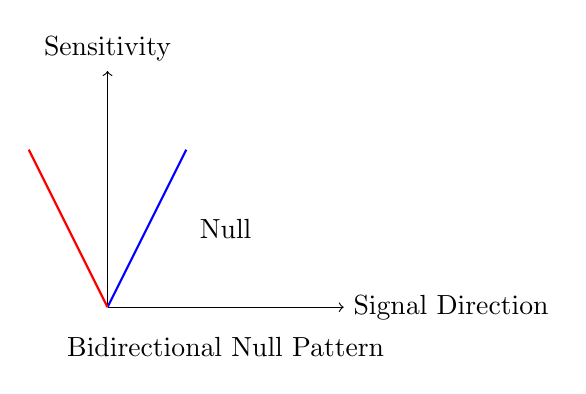
\begin{tikzpicture}
\draw[->] (0,0) -- (3,0) node[right] {Signal Direction};
\draw[->] (0,0) -- (0,3) node[above] {Sensitivity};
\draw[blue,thick] (0,0) -- (1,2);
\draw[red,thick] (0,0) -- (-1,2);
\node at (1.5,1) {Null};
\node[align=center] at (1.5,-0.5) {Bidirectional Null Pattern};
\end{tikzpicture}
\end{center}
